\documentclass[UTF8]{ctexbook}
\usepackage[a4paper, left = 3cm, right = 3cm, top = 3cm, bottom = 3cm]{geometry}
\usepackage{amsmath} % 数学公式
\usepackage{amssymb}             % 数学公式
\usepackage{amsfonts}            % 数学字体
\usepackage{mathrsfs}            % 数学花体
\usepackage{graphicx}
\usepackage{color}
\usepackage{framed}

\usepackage{theorem} % 定理
\theoremheaderfont{\sffamily\bfseries}
\theorembodyfont{\normalfont}

\definecolor{shadecolor}{gray}{0.85}
\newcommand{\myref}[1]{\ \ref{#1}\ }
\newtheorem{thm}{定理}[chapter]
\newtheorem{lemma}{引理}[chapter]
\newtheorem{prop}{命题}[chapter]
\newtheorem{definition}{定义}[chapter]
\newenvironment{proof}{
	\begin{shaded}
		\par\noindent{\sffamily\bfseries 证明}
}{
	\hfill\mbox{$\Box$}\end{shaded}
}

\title{积分变换的相关概念}
\author{玩味者}
\begin{document}
	\maketitle
	\tableofcontents
	\chapter{傅里叶变换的理论部分}
    \section{傅里叶级数的复数形式}
        在微积分课程中已经知道,一个周期函数如果满足Dirichlet条件,便可以表达为如下的三角无穷级数形式:
        \begin{equation}
            \begin{split}
                &f(t)=\dfrac{a_0}{2}+\sum_{n = 1}^\infty(a_n\cos n\omega t+b_n\sin n\omega t)\quad t\in [-\dfrac{T}{2}, \dfrac{T}{2}]\\
                &\omega= \dfrac{2\pi}{T},\\
                &a_0=\dfrac{2}{T}\int_{-\frac{T}{2}}^{\frac{T}{2}}f(t)\ dt,\\
                &a_n=\dfrac{2}{T}\int_{-\frac{T}{2}}^{\frac{T}{2}}f(t)\cos n\omega t\ dt,\\
                &b_n=\dfrac{2}{T}\int_{-\frac{T}{2}}^{\frac{T}{2}}f(t)\sin n\omega t\ dt,\\
            \end{split}
            \label{eq: 1.1}
        \end{equation}

        以上的形式称为函数的傅里叶级数展开式(三角形式)。

        一个函数被分解为两种三角函数的无穷和,这种形式的使用是不方便的,如果能变成同一个函数的无穷和,事情就会简单很多。于是引入欧拉公式:
        \begin{equation}
            e^{i\theta}=\cos \theta +i \sin\theta
            \label{eq: 1.2}
        \end{equation}

        \begin{proof}
            以下是欧拉本人的证明思路:假如$e^x$的泰勒展开式在复数域成立,则

            \begin{equation*}
                \begin{split}
                    e^{i\theta}&=1+i\theta+\dfrac{(i\theta)^2}{2!}+\dfrac{(i\theta)^3}{3!}+\dfrac{(i\theta)^3}{3!}+\cdots\\
                    &=(1 - \dfrac{\theta^2}{2!} + \dfrac{\theta^4}{4!} - \cdots) + (i\theta - \dfrac{i\theta^3}{3!} + \dfrac{\theta^5}{5!} - \cdots)\\
                    &=\cos \theta + i\sin \theta
                \end{split}
            \end{equation*}
        \end{proof}

        由\myref{eq: 1.2}式可以很容易推导出
        \begin{equation}
            \cos\theta =\dfrac{e^{i\theta}+e^{-i\theta}}{2}\quad \sin\theta = \dfrac{e^{i\theta}-e^{-i\theta}}{2i}
            \label{eq: 1.3}
        \end{equation}

        将\myref{eq: 1.3}代入\myref{eq: 1.1}
        \begin{equation}
            \begin{split}
                f(t)&=\dfrac{a_0}{2}+\sum\limits_{n = 1}^\infty(a_n\dfrac{e^{in\omega t}+e^{-in\omega t}}{2}+b_n\dfrac{e^{in\omega t}-e^{-in\omega t}}{2i})\\
                &= \dfrac{a_0}{2}+\sum\limits_{n = 1}^\infty(\dfrac{a_n-i b_n}{2}e^{in\omega t}+\dfrac{a_n+i b_n}{2}e^{-in\omega t})
            \end{split}
            \label{eq: 1.4}
        \end{equation}
        
        根据傅里叶系数的三角形式和\myref{eq: 1.2}的比较,可以知道
        \begin{equation}
            \begin{split}
                &\begin{split}
                    a_n+ib_n&=\dfrac{2}{T}\int_{-\frac{T}{2}}^{\frac{T}{2}}f(t)\cos n\omega t\ dt+i\dfrac{2}{T}\int_{-\frac{T}{2}}^{\frac{T}{2}}f(t)\sin n\omega t\ dt\\
                    &= \dfrac{2}{T}\int_{-\frac{T}{2}}^{\frac{T}{2}}f(t)(\cos n\omega t+i\sin n\omega t)\ dt\\
                    &= \dfrac{2}{T}\int_{-\frac{T}{2}}^{\frac{T}{2}}f(t)e^{in\omega t}\ dt
                \end{split}\\
                &a_n-ib_n=\dfrac{2}{T}\int_{-\frac{T}{2}}^{\frac{T}{2}}f(t)e^{-in\omega t}\ dt
            \end{split}
            \label{eq: 1.5}
        \end{equation}

        $n=0$时,\myref{eq: 1.5}式将退化为\myref{eq: 1.1}式中$a_0$的形式,令
        \begin{equation}
            c_n=\dfrac{1}{T}\int_{-\frac{T}{2}}^{\frac{T}{2}}f(t)e^{-in\omega t}\ dt, \quad \omega_n=n\omega
            \label{eq: 1.6}
        \end{equation}

        这样就可以把三角形式的系数全部转成
        \begin{equation}
            \dfrac{a_0}{2}=c_0,\quad
            \dfrac{a_n+ib_n}{2}=c_{-n},\quad
            \dfrac{a_n-ib_n}{2}=c_{n}
            \label{eq: 1.7}
        \end{equation}

        所以
        \begin{equation}
            \begin{split}
                f(t)&= c_0+\sum\limits_{n=1}^\infty[c_n e^{i\omega_n t}+c_{-n}e^{i\omega_{-n} t}]\\
                &= \sum\limits_{n=-\infty}^{\infty}c_n e^{i\omega_n t}
            \end{split}
            \label{eq: 1.8}
        \end{equation}

        于是,结合\myref{eq: 1.8}和\myref{eq: 1.6},我们得到了\textbf{傅里叶级数的复数形式}\footnote{其实,非周期函数可以看作是周期为$[-\infty, \infty]$的周期函数,此时,任意函数(这里并不严格)都可以满足(1.8)式}

    \section{傅里叶积分公式}
        当周期$T$无穷大的时候,有
        \begin{equation}
            \lim_{T\to +\infty}f_T(t)=f(t)
            \label{eq: 1.9}
        \end{equation}
        那么,根据\myref{eq: 1.8}式,一个非周期函数$f(t)$就有
        \begin{equation}
            f(t)=\lim_{T\to +\infty}\sum\limits_{n=-\infty}^{\infty}\left[\dfrac{1}{T}\int_{-\frac{T}{2}}^{\frac{T}{2}}f(\tau)e^{-i\omega_n \tau}\ d\tau\right] e^{i\omega_n t}
            \label{eq: 1.10}
        \end{equation}

        当$n$取一切整数的时候,$\omega_n$所对应的点便均匀地分布在整个数轴上
        \begin{equation}
            \Delta\omega_n=\omega_n-\omega_{n - 1}=\dfrac{2\pi}{T}\Rightarrow T=\dfrac{2\pi}{\Delta\omega_n}
            \label{eq: 1.11}
        \end{equation}
        
        当$T\to +\infty$时,$\Delta\omega_n\to 0$,所以(1.10)可以写作
        \begin{equation}
            f(t)=\lim_{\Delta\omega_n\to 0}\sum\limits_{n=-\infty}^{\infty}\left[\dfrac{1}{2\pi}\left(\int_{-\infty}^{\infty}f(\tau)e^{-i\omega_n \tau}\ d\tau\right)e^{i\omega_n t}\right] \Delta\omega_n
            \label{eq: 1.12}
        \end{equation}
        
        把式子排列成上面这种形式是有原因的,把中括号内部的部分看作是一个关于$\omega_n$的函数,那么整个式子正好是定积分的定义式,于是(12)式可以写成下面的形式
        \begin{equation}
            f(t)=\dfrac{1}{2\pi}\int_{-\infty}^{\infty}\left[\int_{-\infty}^{\infty}f(\tau)e^{-i\omega \tau}\ d\tau\right] e^{i\omega t} d\omega
            \label{eq: 1.13}
        \end{equation}
        
        将\myref{eq: 1.13}式称为\textbf{傅里叶积分公式}

    \section{傅里叶变换}

        由\myref{eq: 1.13}式可以直接得出傅里叶变换的形式,设中括号内部的部分为
        \begin{equation}
            F(\omega)=\int_{-\infty}^{\infty}f(t)e^{-i\omega t}\ dt
            \label{eq: 1.14}
        \end{equation}

        那么,把\myref{eq: 1.14}代入\myref{eq: 1.13}
        \begin{equation}
            f(t)=\dfrac{1}{2\pi}\int_{-\infty}^{\infty}F(\omega) e^{i\omega t} d\omega
            \label{eq: 1.15}
        \end{equation}

        这里,\myref{eq: 1.14}被称为$f(t)$的\textbf{傅里叶变换式}\footnote{当然,在工程中也有使用如下形式的傅里叶变换
            $$
            F(\omega)=\sqrt{\dfrac{1}{2\pi}}\int_{-\infty}^{\infty}f(t)e^{-i\omega t}\ dt\\
            f(t)=\sqrt{\dfrac{1}{2\pi}}\int_{-\infty}^{\infty}F(\omega) e^{i\omega t} d\omega
            $$
            这样可以使得系数均衡(强迫症福利),这个都是人为定义的,系数的改变并不影响其数学性质},记作
        \begin{equation}
            F(\omega)=\mathscr{F}[f(t)]
            \label{eq: 1.16}
        \end{equation}

        反之,\myref{eq: 1.15}被称为$F(\omega)$的\textbf{傅里叶逆变换式},记作
        \begin{equation}
            f(t)=\mathscr{F}^{-1}[F(\omega)]
            \label{eq: 1.17}
        \end{equation}
        
        在信号处理的时候,一个连续的信号可以看作是$f(t)$,这是以时间为自变量的函数,而它的傅里叶变换$F(\omega)$是以$\omega$为自变量的函数,或者说,是频率的函数($\omega=2\pi f$)

    \section{傅里叶变换的性质}

        傅里叶变换的形式是很美好的,简单明了。但是要应用这个结论,需要找到它的一些性质。以下讨论都假设$f(t)$是符合傅里叶变换要求的函数

        \begin{enumerate}
            \item{线性性质}
                由于积分的线性性质,傅里叶变换很自然也具有线性性质
                \begin{equation}
                    \begin{split}
                        &\mathscr{F}[\alpha f_1(t)+\beta f_2(t)] = \alpha F_1(\omega)+\beta F_2(\omega)\\
                        &\mathscr{F}^{-1}[\alpha F_1(\omega)+\beta F_2(\omega)] = \alpha f_1(t)+\beta f_2(t)
                    \end{split}
                    \label{eq: 1.18}
                \end{equation}

            \item{位移性质}
                \begin{equation}
                    \begin{split}
                        &\begin{split}
                            \mathscr{F}[f(t\pm t_0)]&=\int_{-\infty}^{\infty}f(t\pm t_0)e^{-i\omega t}\ dt\\
                            &= \int_{-\infty}^{\infty}f(u)e^{-i\omega (u\mp t_0)}\ du\\
                            &= e^{\pm i\omega t_0}\int_{-\infty}^{\infty}f(u)e^{-i\omega u}\ du\\
                            &= e^{\pm i\omega t_0}F(\omega)
                        \end{split}\\
                        &\mathscr{F}^{-1}[F(\omega\mp\omega_0)]=e^{\pm i\omega_0 t}f(t)
                    \end{split}
                    \label{eq: 1.19}
                \end{equation}
                上面的这个结论说明,函数在时域或频域上的位移相当于相对的域中的函数乘以一个因子(加减$\to$乘除)

            \item{微分性质}
                \begin{equation}
                    \begin{split}
                        \mathscr{F}[f'(t)]&=\int_{-\infty}^{\infty}f'(t)e^{-i\omega t}\ dt\\
                        &=\int_{-\infty}^{\infty}e^{-i\omega t}\ df(t)\\
                        &=f(t)e^{-i\omega t}|_{-\infty}^{\infty}-\int_{-\infty}^{\infty}f(t)\ de^{-i\omega t}\\
                        &=f(t)e^{-i\omega t}|_{-\infty}^{\infty}+i\omega\int_{-\infty}^{\infty}f(t)e^{-i\omega t}\ dt\\
                    \end{split}
                    \label{eq: 1.20}
                \end{equation}
                做到这一步做不下去了,因为如果不给$f(t)$再加上额外的限制的话,$f(t)e^{-i\omega t}|_{-\infty}^{\infty}$这一项就会变成无穷大,所以,必须给$f(t)$加一个限制
    
                \begin{quote}
                    $f(t)$在$(-\infty, \infty)$上连续或只有有限个可去间断点,且当$|t|\to +\infty$时,$f(t)\to 0$
                \end{quote}
    
                有了这个限制之后,前面那一项等于0,得到
                \begin{equation}
                    \begin{split}
                    \mathscr{F}[f'(t)]&=i\omega\int_{-\infty}^{\infty}f(t)e^{-i\omega t}\ dt\\
                    &=i\omega\mathscr{F}[f(t)]
                    \end{split}
                    \label{eq: 1.21}
                \end{equation}
    
                用类似的方法(限制条件),可以得到
                \begin{equation}
                    \mathscr{F}^{-1}[F'(\omega)]=-it\mathscr{F}^{-1}[F(\omega)]
                    \label{eq: 1.22}
                \end{equation}
                这个性质是很有用的,它把一个函数的求导变成了对应域中的乘因子
    
                使用数学归纳法可以很容易证明,对于$n$阶微分也有该性质,区别在于对因子求$n$次幂
    
                在求导方便的时候,可以用这种方法来求$t^nf(t)$形式函数的傅里叶变换结果;反之,则可以用傅里叶变换求出导数

            \item{积分性质}
                \begin{equation}
                    \begin{split}
                        \begin{split}
                        \mathscr{F}[f(t)]&=\mathscr{F}[\dfrac{d}{dt}\int_{-\infty}^tf(t)\ dt]\\
                        &= i\omega\mathscr{F}[\int_{-\infty}^tf(t)\ dt]
                        \end{split}\\
                        \Rightarrow\mathscr{F}[\int_{-\infty}^tf(t)\ dt]=\dfrac{1}{i\omega}\mathscr{F}[f(t)]
                    \end{split}
                    \label{eq: 1.23}
                \end{equation}
                同理
                \begin{equation}
                    \mathscr{F}^{-1}[\int_{-\infty}^\omega F(\omega)\ d\omega]=-\dfrac{1}{it}\mathscr{F}^{-1}[F(\omega)]
                    \label{eq: 1.24}
                \end{equation}
                和微分性质类似,这里不再赘述

            \item{乘积定理}
                设$F_1(\omega) = \mathscr{F}[f_1(t)]$,$F_2(\omega) = \mathscr{F}[f_2(t)]$,则
                \begin{equation}
                    \begin{split}
                        &\int_{-\infty}^{\infty}\overline{f_1(t)}f_2(t)dt=\dfrac{1}{2\pi}\int_{-\infty}^{\infty}\overline{F_1(\omega)}F_2(\omega)d\omega\\
                        &\int_{-\infty}^{\infty}f_1(t)\overline{f_2(t)}dt=\dfrac{1}{2\pi}\int_{-\infty}^{\infty}F_1(\omega)\overline{F_2(\omega)}d\omega
                    \end{split}
                    \label{eq: 1.25}
                \end{equation}
                这个结论很有意思,这说明原函数的乘积之积分和变换之后的乘积之积分仅有一个系数的差异(如果按照另外一种傅里叶变换的定义,则这个系数差异也没有)

            \item{能量积分}
                如果在上一个性质中,两个函数一样,那么可以得到
                \begin{equation}
                    \int_{-\infty}^{\infty}[f(t)]^2\ dt=\dfrac{1}{2\pi}\int_{-\infty}^{\infty}|F(\omega)|^2\ d\omega
                    \label{eq: 1.26}
                \end{equation}
                这个结论是非常重要的,称为Parseval等式,令
                \begin{equation}
                    S(\omega)=|F(\omega)|^2
                    \label{eq: 1.27}
                \end{equation}
                称为\textbf{能量密度函数}或\textbf{能量谱密度},由它可以决定函数$f(t)$的能量分布规律
    
                这里说$[f(t)]^2$是能量密度,或者说信号的“功率”,这是需要解释的:
        \end{enumerate}
        \begin{shaded}
            所谓功率,在物理上的定义是单位时间内做功的多少,以如下式定义:
            \begin{equation}
            P = \dfrac{W}{t}
            \label{eq: 1.28}
            \end{equation}
            更进一步,我们假设这个函数是一个电信号的抽象。在电路中:
            \begin{equation}
            P = UI = I^2R = \dfrac{U^2}{R}
            \label{eq: 1.29}
            \end{equation}
            以上面的式子来看,信号幅值的度量是用电压的高低表示的,如果把电路中的电阻值视为单位1,那么输出信号的瞬时功率就是
            \begin{equation}
            P = U^2
            \label{eq: 1.30}
            \end{equation}
            一段时间内的功率就应该对其在时间上积分,所以,用信号的平方表示信号的功率是恰当的
        \end{shaded}

    \section{卷积定理}
        卷积的定义是:
        \begin{equation}
            f_1(t)*f_2(t) = \int_{-\infty}^{+\infty}f_1(\tau)f_2(t - \tau)\ d\tau
            \label{eq: 1.31}
        \end{equation}
        下面结合\myref{eq: 1.14},我们对两个函数的卷积进行傅里叶变换:
        \begin{equation}
            \begin{split}
                \mathscr{F}[f_1(t)*f_2(t)] &= \mathscr{F}[\int_{-\infty}^{+\infty}f_1(\tau)f_2(t - \tau)\ d\tau]\\
                &= \int_{-\infty}^{+\infty}\int_{-\infty}^{+\infty}f_1(\tau)f_2(t - \tau)\ d\tau\ e^{-i\omega t}\ dt\\
                &= \int_{-\infty}^{+\infty}\int_{-\infty}^{+\infty}f_1(\tau)f_2(t - \tau)e^{-i\omega (\tau + t -\tau)}\ d\tau dt\\
                &= \int_{-\infty}^{+\infty}\int_{-\infty}^{+\infty}f_1(\tau)e^{-i\omega \tau}f_2(t - \tau)e^{-i\omega (t - \tau)}\ d\tau dt\\
                &= \int_{-\infty}^{+\infty}\int_{-\infty}^{+\infty}f_1(\tau)e^{-i\omega \tau}f_2(t - \tau)e^{-i\omega (t - \tau)}\ dt d\tau\\
                &= \int_{-\infty}^{+\infty}f_1(\tau)e^{-i\omega \tau}d\tau\int_{-\infty}^{+\infty}f_2(t - \tau)e^{-i\omega (t - \tau)}\ dt\\
                &= \mathscr{F}[f_1(t)]\cdot\mathscr{F}[f_2(t)]
            \end{split}
            \label{eq: 1.32}
        \end{equation}
        同理可得
        \begin{equation}
            \begin{split}
                \mathscr{F}[f_1(t)\cdot f_2(t)] &= \dfrac{1}{2\pi}\int_{-\infty}^{\infty}F_1(\omega) e^{i\omega t} d\omega\ \dfrac{1}{2\pi}\int_{-\infty}^{\infty}F_2(\omega) e^{i\omega t} d\omega\\
                &= \dfrac{1}{(2\pi)^2}\int_{-\infty}^{\infty}F_1(\tau) e^{i\tau t} d\tau\ \int_{-\infty}^{\infty}F_2(\omega - \tau) e^{i(\omega - \tau) t} d(\omega - \tau)\\
                &= \dfrac{1}{(2\pi)^2}\int_{-\infty}^{\infty}\int_{-\infty}^{\infty}F_1(\tau) e^{i\tau t} F_2(\omega - \tau) e^{i(\omega - \tau) t}\ d\tau d\omega\\
                &= \dfrac{1}{(2\pi)^2}\int_{-\infty}^{\infty}\left[\int_{-\infty}^{\infty}F_1(\tau) F_2(\omega - \tau)\ d\tau\right]e^{i\omega t}d\omega\\
                &= \dfrac{1}{(2\pi)^2}\int_{-\infty}^{\infty}\left[F_1(\omega)*F_2(\omega)\right]e^{i\omega t}d\omega\\
                &= \dfrac{1}{2\pi}\mathscr[F_1(\omega)*F_2(\omega)]
            \end{split}
            \label{eq: 1.33}
        \end{equation}
        我们称\myref{eq: 1.32}式为\textbf{时域的卷积定理},称\myref{eq: 1.33}式为\textbf{频域的卷积定理}

    \section{频谱的意义}
        结合傅里叶积分公式\myref{eq: 1.13}以及傅里叶级数的复数形式\myref{eq: 1.8}可以看到,所谓的频域函数$F(\omega)$其实是无穷级数中的系数$c_n$,唯一的一串$c_n$序列决定了一个周期函数$f(t)$,而$c_n$中含有一个完整的正弦函数(谐波)。从\myref{eq: 1.1}式中可以知道,某一个周期函数的第n次谐波为
        \begin{equation}
            a_n\cos \omega_n t+b_n\sin\omega_n t=A_n\sin(\omega_n t + \varphi_n)
            \label{eq: 1.34}
        \end{equation}

        其中
        \begin{equation}
            A_n = \sqrt{a_n^2+b_n^2}
            \label{eq: 1.35}
        \end{equation}

        从\myref{eq: 1.8}式中的傅里叶变换的复数形式中我们又可以知道,第n次谐波为
        \begin{equation}
            c_ne^{i\omega_nt}+c_{-n}e^{i\omega_{-n}t}
            \label{eq: 1.36}
        \end{equation}

        其中
        \begin{equation}
            c_n=\dfrac{a_i-ib_n}{2}\quad c_{-n} = \dfrac{a_n + ib_n}{2}
            \label{eq: 1.37}
        \end{equation}

        从上式可以知道
        \begin{equation}
            |c_n| = |c_{-n}| = \dfrac 1 2 A_n
            \label{eq: 1.38}
        \end{equation}

        所以说,$F(\omega)$的模长(作为一个复变函数来看)代表了原函数每一个谐波的振幅
        
        正如之前推导傅里叶积分公式时所做的那样,一个非周期函数可以视为一个最小正周期无穷大的周期函数。一旦我们这样做了以后,每两个$\omega$之间的距离就变得无穷小,那么频率域的函数就是一个连续函数了
        
        得到了上面的结论之后就可以知道,$F(\omega)$是频谱函数,而$|F(\omega)|$是振幅函数

	\chapter{一些特殊函数的傅里叶变换}
    \section{方波}
        \begin{equation}
            f(t)=E, \quad t\in \left[-\frac{\tau}{2}, \frac{\tau}{2}\right]
            \label{eq: 2.1}
        \end{equation}
        下面求$f(t)$的傅里叶变换结果
        \begin{equation}
            \begin{split}
                \mathscr{F}[f(t)] &= \int_{-\infty}^{\infty}f(t)e^{-i\omega t}\ dt\\
                &= \int_{-\infty}^{\infty}E\ e^{-i\omega t}\ dt\\
                &= -\dfrac{E}{i\omega}e^{-i\omega t}|_{-\frac{\tau}{2}}^{\frac{\tau}{2}}\\
                &= \dfrac{E}{i\omega}(e^{i\omega \frac{\tau}{2}}-e^{-i\omega\frac{\tau}{2}})\\
            \end{split}
            \label{eq: 2.2}
        \end{equation}
        上式利用欧拉定理\myref{eq: 1.2},得到
        \begin{equation}
            \begin{split}
                \mathscr{F}[f(t)] &= \dfrac{E}{i\omega}(e^{i\omega \frac{\tau}{2}}-e^{-i\omega\frac{\tau}{2}})\\
                &= \dfrac{E}{i\omega}(\cos (\omega \dfrac{\tau}{2}) +i \sin(\omega \dfrac{\tau}{2})-\cos (-\omega \dfrac{\tau}{2}) -i \sin(-\omega \dfrac{\tau}{2}))\\
                &= \dfrac{E}{i\omega}(i \sin(\omega \dfrac{\tau}{2}) +i \sin(\omega \dfrac{\tau}{2}))\\
                &= \dfrac{2E}{\omega}\sin\dfrac{\omega\tau}{2}\\
            \end{split}
            \label{eq: 2.3}
        \end{equation}
        图\myref{fig: 2.1}是由Mathematica生成的图像,表示$E = 1, \tau = 1$时的图像
        
        \begin{figure}[h]
            \centering
            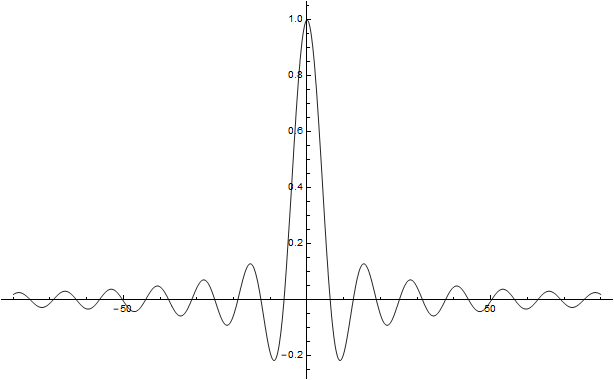
\includegraphics[scale=0.3]{1.png}
            \caption{方波的傅里叶变换}
            \label{fig: 2.1}
        \end{figure}

        应当注意到,这个函数是$\dfrac{\sin x}{x}$的变形,在$x=0$的时候是没有定义的

    \section{$\delta$-函数}

        这是一种广义的函数由一个描述和一个积分式共同定义
        \begin{equation}
            \delta(t) = \left\{
            \begin{aligned}
            \infty & \qquad t=0\\
            0& \qquad else 
            \end{aligned}
            \right.
            \label{eq: 2.4}
        \end{equation}
        并且
        \begin{equation}
            \int_{-\infty}^{\infty}\delta(t)\ dt=\int_{0}^{\epsilon}\dfrac{1}{\epsilon}\ dt=1
            \label{eq: 2.5}
        \end{equation}

        这个函数没办法用图像表示出来,因为它在$t = 0$的时候有一个无穷大的冲激,而在其他地方值为0,就好像用钉子钉墙,一个能量恒定的冲激作用在一个面积很小的点上,而其他的地方则没有能量作用。故这个函数又叫做冲激函数。

        下面证明,$\delta$-函数具有采样性质:
        \begin{equation}
            \int_{-\infty}^{\infty}\delta(t-t_0)f(t)\ dt=f(t_0)
            \label{eq: 2.6}
        \end{equation}

        \begin{proof}
            设$f(t)$是一个在$t_0$处连续的函数
            \begin{equation}
                \int_{-\infty}^{\infty}\delta(t-t_0)f(t)\ dt = \lim_{\epsilon\to 0}\dfrac{1}{\epsilon}\int_{t_0}^{t_0+\epsilon}f(t)\ dt
                \label{eq: 2.7}
            \end{equation}
            
            利用积分中值定理
            \begin{equation}
                \int_{a}^{b}f(x)\ dx = f(\epsilon) (b - a)\qquad a\leq\epsilon\leq b
                \label{eq: 2.8}
            \end{equation}
            可以得到
            \begin{equation}
                \int_{-\infty}^{\infty}\delta(t-t_0)f(t)\ dt = f(\tau)\qquad \tau\in\left[t_0, t_0 + \epsilon\right]
                \label{eq: 2.9}
            \end{equation}
            由于$\epsilon\to 0$,所以
            \begin{equation}
                \int_{-\infty}^{\infty}\delta(t-t_0)f(t)\ dt = f(t_0)
                \label{eq: 2.10}
            \end{equation}
            
            命题得证
        \end{proof}

        证明了这个性质之后,它的傅里叶变换便可以直接得出来:
        \begin{equation}
            \mathscr{F}[\delta(t)]=\int_{-\infty}^{\infty}\delta(t)e^{-i\omega t}\ dt=1
            \label{eq: 2.11}
        \end{equation}


    \section{阶跃函数}
        \begin{definition}
            \begin{equation}
                \epsilon(t)=\left\{
                \begin{aligned}
                0&\qquad t<0\\
                1&\qquad t>0
                \end{aligned}
                \right.
                \label{eq: 2.12}
            \end{equation}
        \end{definition}
        根据定义我们可以知道,阶跃函数的微分即$\delta$-函数

        这里要说明的是,对于阶跃函数的傅里叶变换结果的得出需要使用广义函数的知识,所以这里先给出结果,然后反向证明其正确。
        \begin{equation}
            \mathscr{F}[\epsilon(t)]=\dfrac{1}{i\omega}+\pi\delta(\omega)
            \label{eq: 2.13}
        \end{equation}
        
        为了证明这个式子,需要先证明三个引理:

        \begin{lemma}
            \begin{equation}
                \int \dfrac{1}{x^2 + 1}\ dx=\arctan x+c
                \label{eq: 2.14}
            \end{equation}
        \end{lemma}

        \begin{proof}
            令$\tan y = x$,则
            \begin{equation*}
                \begin{split}
                    \dfrac{dx}{dy}&=\dfrac{d(\tan y)}{dy}\\
                    &=\dfrac{d(\frac{\sin y}{\cos y})}{dy}\\
                    &=\dfrac{\sin^2 y+\cos^2 y}{\cos^2 y}\\
                    &=\tan^2 y+1\\
                    &=x^2+1
                \end{split}
            \end{equation*}
            
            所以
            \begin{equation*}
                \dfrac{dy}{dx}=\dfrac{1}{x^2+1}\Rightarrow\int \dfrac{1}{x^2 + 1}\ dx=\arctan x+c
            \end{equation*}

            证毕
        \end{proof}
        \begin{lemma}
            \begin{equation}
                \int_{0}^{\infty}\sin x e^{-ax}\ dx=\dfrac{1}{a^2+1}
                \label{eq: 2.15}
            \end{equation}
        \end{lemma}
        \begin{proof}
            令
            \begin{equation*}
                I=\int_{0}^{\infty}\sin x e^{-ax}\ dx
            \end{equation*}
            
            则
            \begin{equation*}
                \begin{split}
                    &-I=e^{-ax}\cos x\bigg|_{0}^{\infty}+\int_{0}^{\infty}a\cos x e^{-ax}\ dx\\
                    &\Rightarrow -I=-1+a\int_{0}^{\infty}\cos x e^{-ax}\ dx\\
                    &\Rightarrow \dfrac{1-I}{a}=\int_{0}^{\infty} e^{-ax}\ d\sin x\\
                    &\Rightarrow \dfrac{1-I}{a}=e^{-ax}\sin x\bigg|_{0}^{\infty}+\int_{0}^{\infty} a\sin x e^{-ax}\ dx\\
                    &\Rightarrow \dfrac{1-I}{a}=0+aI\\
                    &\Rightarrow I=\dfrac{1}{a^2+1}\\
                \end{split}
            \end{equation*}

            证毕
        \end{proof}

        \begin{lemma}{Dirichlet积分}
            \begin{equation}
                \int_{0}^{\infty}\dfrac{\sin x}{x}\ dx=\dfrac{\pi}{2}
                \label{eq: 2.16}
            \end{equation}
        \end{lemma}

        我们知道,这个函数在零点是无意义的,而且它的积分是一个反常积分,只有无穷级数形式,没有解析表达式,这就导致求它的积分需要特殊的方法

        下面分别用\emph{多重积分}和\emph{费曼技巧}两种证明方法对该结论进行证明

        \begin{proof}
            令
            \begin{equation*}
                \begin{split}
                    I_1=\int_{0}^{\infty}\int_{0}^{\infty}e^{-xy}\sin y\ dxdy\\
                    I_2=\int_{0}^{\infty}\int_{0}^{\infty}e^{-xy}\sin y\ dydx
                \end{split}
            \end{equation*}

            由于这两个二重积分仅仅是积分次序不用,所以很显然有$I_1=I_2$,并且由$I_1$得到:
            \begin{equation*}
                \begin{split}
                    I_1&=\int_{0}^{\infty}\sin y(\int_{0}^{\infty}e^{-xy}\ dx)dy\\
                    &=\int_{0}^{\infty}\sin y(-\frac{1}{y}e^{-xy})\big|_0^\infty dy\\
                    &=\int_{0}^{\infty}\dfrac{\sin y}{y} dy\\
                \end{split}
            \end{equation*}

            由\myref{eq: 2.14}和\myref{eq: 2.15}可以得到
            \begin{equation*}
                I_2=\int_{0}^{\infty}\dfrac{1}{x^2+1}\ dx=\arctan x\bigg|_{0}^{\infty}=\dfrac{\pi}{2}\tag*{}
            \end{equation*}

            由$I_1=I_2$得到结果,证毕.
        \end{proof}

        下面的方法被称为\emph{费曼技巧},这是一种求定积分的有效方法,由理查德·费曼使用并推广,简要来说叫做“积分内取微分”

        \begin{proof}
            令
            \begin{equation*}
                I(a)=\int_{0}^{\infty}\dfrac{\sin x}{x}e^{-ax}\ dx
            \end{equation*}

            将该函数对变量$a$取微分
            \begin{equation*}
                \begin{split}
                    &\dfrac{dI(a)}{da}=\int_{0}^{\infty}-x\dfrac{\sin x}{x}e^{-ax}\ dx\\
                    &\Rightarrow \dfrac{dI(a)}{da}=-\int_{0}^{\infty}\sin x e^{-ax}\ dx=-\dfrac{1}{a^2+1}
                \end{split}
            \end{equation*}

            对上述结果再取定积分
            \begin{equation*}
                \begin{split}
                    &\int_{0}^{\infty}-\dfrac{1}{a^2+1}\ dx=I(\infty)-I(0)\\
                    &\Rightarrow -\dfrac{\pi}{2}=-I(0)\\
                    &\Rightarrow\int_{0}^{\infty}\dfrac{\sin x}{x}\ dx=\dfrac{\pi}{2}
                \end{split}
            \end{equation*}

            证毕
        \end{proof}

        证明了上面的三个引理之后,可以来证明结论了:
        \begin{proof}
            假如命题正确,则有
            \begin{equation*}
                \begin{split}
                    \epsilon(t)&=\mathscr{F}^{-1}[\dfrac{1}{i\omega}+\pi\delta(\omega)]\\
                    &=\dfrac{1}{2\pi}\int_{-\infty}^{\infty}[\dfrac{1}{i\omega}+\pi\delta(\omega)] e^{i\omega t} d\omega\\
                    &=\dfrac{1}{2\pi}\int_{-\infty}^{\infty}\dfrac{1}{i\omega} e^{i\omega t} d\omega+\dfrac{1}{2\pi}\int_{-\infty}^{\infty}\pi\delta(\omega) e^{i\omega t} d\omega\\
                    &=\dfrac{1}{2\pi}\int_{-\infty}^{\infty}\dfrac{1}{i\omega} (\cos \omega t +i \sin\omega t)\ d\omega+\dfrac{1}{2}\\
                    &=\dfrac{1}{\pi}\int_{0}^{\infty}\dfrac{\sin\omega t}{\omega}\ d\omega+\dfrac{1}{2}\\
                \end{split}
            \end{equation*}

            由\myref{eq: 2.16}我们知道,$\int_{0}^{\infty}\dfrac{\sin\omega}{\omega}\ d\omega=\dfrac{\pi}{2}$,由于$t\omega\sim\omega$,故存在下列关系
            \begin{equation*}
                \int_{0}^{\infty}\dfrac{\sin\omega t}{\omega}\ d\omega=\left\{\begin{aligned}
                -\frac{\pi}{2}&\qquad t<0\\
                0&\qquad t=0\\
                \dfrac{\pi}{2}&\qquad t>0
                \end{aligned}\right.
            \end{equation*}

            故
            \begin{equation*}
                \epsilon(t)=\left\{\begin{aligned}
                \dfrac 1 2 + \dfrac \pi 2(-\frac{\pi}{2})&\qquad t<0\\
                \dfrac 1 2 + \dfrac \pi 2(\dfrac{\pi}{2})&\qquad t>0
                \end{aligned}\right.\Rightarrow\left\{\begin{aligned}
                0&\qquad t<0\\
                1&\qquad t>0
                \end{aligned}\right.
            \end{equation*}

            这正是阶跃函数,所以命题成立
        \end{proof}
    \section{1}
        以上面这种先入为主的方式,我们再来捡几个傅里叶变换对:
        \begin{equation}
            \mathscr{F}[1]=2\pi\delta(\omega)
            \label{eq: 2.17}
        \end{equation}
        \begin{proof}
            \begin{equation*}
                \mathscr{F}^{-1}[2\pi\delta(\omega)]=\dfrac{1}{2\pi}\int_{-\infty}^{\infty}2\pi\delta(\omega)e^{i\omega t}\ d\omega=1\tag*{}
            \end{equation*}
            证毕
        \end{proof}

        结合\myref{eq: 2.11},发现这其实是两对傅里叶变换对
    \section{指数函数}
        \begin{equation}
            \mathscr{F}[e^{i\omega_0 t}]=2\pi\delta(\omega-\omega_0)
            \label{eq: 2.18}
        \end{equation}
        \begin{proof}
            \begin{equation*}
                \begin{split}
                    &\mathscr{F}^{-1}[2\pi\delta(\omega-\omega_0)]=\dfrac{1}{2\pi}\int_{-\infty}^{\infty}2\pi\delta(\omega-\omega_0)e^{i\omega t}\ d\omega\\
                    &=\int_{-\infty}^{\infty}\delta(\omega-\omega_0)e^{i(\omega-\omega_0) t}\ d(\omega-\omega_0)\cdot e^{i\omega_0 t}\\
                    &=e^{i\omega_0 t}
                \end{split}
            \end{equation*}
            证毕
        \end{proof}
    \section{正弦函数}
        有了以上的几个傅里叶变换对之后,就可以很容易地求出其他的傅里叶变换,比如正弦函数:
        \begin{equation}
            \begin{split}
                \mathscr{F}[\sin \omega_0t]&=\int_{-\infty}^{\infty}\sin(\omega_0t)e^{-i\omega t}\ dt\\
                &=\int_{-\infty}^{\infty}\dfrac{e^{i\omega_0t}-e^{-i\omega_0t}}{2i}e^{-i\omega t}\ dt\\
                &=\dfrac{1}{2i}\int_{-\infty}^{\infty}(e^{i\omega_0t}-e^{-i\omega_0t})e^{-i\omega t}\ dt\\
                &=\dfrac{1}{2i}\int_{-\infty}^{\infty}(e^{-i(\omega - \omega_0)t}-e^{-i(\omega  + \omega_0)t})\ dt\\
                &=\dfrac{1}{2i}(\mathscr{F}[e^{i\omega_0 t}]-\mathscr{F}[e^{-i\omega_0 t}])\\
                &=\dfrac{1}{2i}(2\pi\delta(\omega-\omega_0)-2\pi\delta(\omega+\omega_0))\\
                &=i\pi(\delta(\omega+\omega_0)-\delta(\omega-\omega_0))\\
            \end{split}
            \label{eq: 2.19}
        \end{equation}
    \section{指数衰减函数}
        \begin{equation}
            f(t)=\left\{\begin{aligned}
            0&\qquad t<0\\
            e^{-\beta t}&\qquad t\geq0
            \end{aligned}
            \right.(\beta>0)
            \label{eq: 2.20}
        \end{equation}

        它的傅里叶变换不需要广义函数加持
        \begin{equation}
            \begin{split}
                \mathscr{F}[f(t)]&= \int_{-\infty}^{\infty}f(t)e^{-i\omega t}\ dt\\
                &= \int_{0}^{\infty}e^{-\beta t}e^{-i\omega t}\ dt\\
                &= \int_{0}^{\infty}e^{-(\beta + i\omega) t}\ dt\\
                &= \dfrac{1}{\beta+i\omega}=\dfrac{\beta-i\omega}{\beta^2+\omega^2}
            \end{split}
            \label{eq: 2.21}
        \end{equation}
    \section{一些思考}
        从上面的结果可以看到,$\delta$-函数可以用来组成所有的非周期函数的傅里叶变换,这一点非常有用

        下面来总结一下刚刚得到的几个傅里叶变换对
        
        \[
            \begin{array}{|c|c|}
                \hline
                \text{时域} & \text{频域}\\ \hline
                E & \frac{2E}{\omega}\sin\frac{\omega\tau}{2}\\ \hline
                \delta(t) & 1\\ \hline
                \epsilon(t) & \frac{1}{i\omega}+\pi\delta(\omega)\\ \hline
                1 & 2\pi\delta(\omega)\\ \hline
                e^{i\omega_0 t} & 2\pi\delta(\omega-\omega_0)\\ \hline
                \sin \omega_0t & i\pi(\delta(\omega+\omega_0)-\delta(\omega-\omega_0))\\ \hline
                e^{-\beta t}\quad t\geq0 & \dfrac{\beta-i\omega}{\beta^2+\omega^2}\\ \hline
            \end{array}
        \]
	\chapter{重温傅里叶级数}
    在第一章中,我们从傅里叶级数开始推导出傅里叶积分公式以及傅里叶变换。但是,这样的推导在数学上是不完整的。下面试图从另一个更加基础的方面来诠释傅里叶级数理论。
    \section{从周期性开始}
        傅里叶级数源于傅里叶的一个简单的想法:\emph{任何}函数都可以表示成一组正弦函数的有限和。当然,从数学分析的角度来说,这样的说法是相当不严谨的,但我们不%
        妨暂时承认这个假设,看看能够走到多远。
        假设一个函数$f(t)$可以表示成一串正弦函数的和,那么
        \begin{equation*}
            f(t) = \sum_{n = 1}^{N} A_n\sin(2\pi n t + \varphi_n)
        \end{equation*}
        但是这个式子很不好看,虽然三个变量可以唯一地决定一个正弦函数,但是在计算的时候,将会遇到很多的障碍(正弦内有加减)。所以,通常将上式变换一下:
        \begin{equation}
            \begin{split}
                A_n\sin(2\pi n t + \varphi_n) &= A_n(\sin(2\pi nt)\cos\varphi_n + \cos(2\pi nt)\sin\varphi_n)\\
                &= (A_n\cos\varphi_n)\sin(2\pi nt) + (A_n\sin\varphi_n)\cos(2\pi nt)\\
                &= a_n\cos(2\pi nt) + b_n\sin(2\pi nt)
            \end{split}
            \label{eq: 3.1}
        \end{equation}
        这里按照习惯,将$\cos(2\pi nt)$放在前面,是无关紧要的。

        但上面的式子有一个不能表示的函数,那就是常函数,所以,可以在这个级数的前面加上一个常数项。至于这个常数项到底是多少,其实是很难判断的。由于$n = 0$时,%
        \myref{eq: 3.1}的结果是$a_0$,所以暂且将常数项定为$ka_0$($k$为系数),于是:
        \begin{equation}
            f(t) = ka_0 + \sum_{n = 1}^{N} a_n\cos(2\pi nt) + b_n\sin(2\pi nt)
            \label{eq: 3.2}
        \end{equation}
        正如我们在第一章中推导过的,通过欧拉公式的变换,可以将上面的这个级数变成
        \begin{equation*}
            \begin{split}
                f(t) &= ka_0 + \sum_{n = 1}^{N} a_n\cos(2\pi nt) + b_n\sin(2\pi nt)\\
                &= ka_0 + \sum_{n = 1}^{N} a_n\dfrac{e^{i2\pi nt} + e^{-i2\pi nt}}{2} + b_n\dfrac{e^{i2\pi nt} - e^{-i2\pi nt}}{2i}\\
                &= ka_0 + \sum_{n = 1}^{N} \frac 1 2 (a_n - ib_n)e^{i2\pi nt} + \frac 1 2 (a_n + ib_n) e^{-i2\pi nt}\\
                &= ka_0 + \sum_{n = 1}^{N} c_n e^{i2\pi nt} + c_{-n} e^{-i2\pi nt}
            \end{split}
        \end{equation*}
        从上面的推导可以看出,如果$k = \frac 1 2$的话,那将是比较合理的,可以将所有的$c_n$合并起来
        \begin{equation}
            f(t) = \sum_{n = -N}^{N} c_n e^{i2\pi nt}
            \label{eq: 3.3}
        \end{equation}
        注意到,$c_n = \overline{c_{-n}}$,$e^{i2\pi nt} = \overline{e^{-i2\pi nt}}$,所以,这个级数是关于实轴对称的。由于共轭复数的和是两倍的实部,%
        那么,\myref{eq: 3.3}就应该是一个实函数:
        \begin{equation*}
            \sum_{n = -N}^{N} c_n e^{i2\pi nt} = c_0 + 2Re\left\{\sum_{n = 1}^{N} c_n e^{i2\pi nt}\right\}
        \end{equation*}
        这样就大可放心了,$f(t)$是一个实变函数,经过一个复数的变换还是一个实变函数,不会跑到复数域去。

        \myref{eq: 3.3}的结论是一个优美的结论,但是这一切都源于对一个假设的默认:任何函数都可以表示成一组正弦函数的有限和。既然我们通过这个假设得到%
        了\myref{eq: 3.3},那就要对这个假设负责,解决下面两个问题:

        \begin{enumerate}
            \item $c_k$的值如何构造,是什么?
            \item $\sum\limits_{n = -N}^{N} c_n e^{i2\pi nt}$真的可以趋近$f(t)$吗?如果可以,它趋近的速度如何?
        \end{enumerate}
        在下一节中,我们将重点解决这两个问题。
\end{document}